\documentclass[addpoints]{exam}

\usepackage[english]{babel}
\usepackage[utf8x]{inputenc}
\usepackage{listings}
\usepackage{amsmath}
\usepackage{amsfonts}
\usepackage{mathtools}
\usepackage{tikz}
\usepackage{qtree}
\usepackage{tikz-qtree}
\usepackage{graphicx}
\usepackage{enumitem}
\usepackage[norelsize,noline,noend,linesnumbered]{algorithm2e}
\usetikzlibrary{arrows,automata}
\usepackage{hyperref}
\hypersetup{
    colorlinks=true,
    linkcolor=blue,
    filecolor=magenta,
    urlcolor=cyan,
}
\usepackage{mdframed}


\begin{document}

\title{CS260 - Written Assignment 3}
\author{Sri Srikanth}
\date{Summer 2024-25}
\maketitle



\newcommand{\limn}{\lim_{n \to \infty}}

\begin{itemize}
\item {\color{red} \textbf{For any algorithm design questions in this assignment and the course as a whole, give your algorithms in C/Python-like pseudocode \textit{and} describe your algorithm briefly at a high level in plain English.}}
\item Your pseudocode can omit low-level details like memory allocations and type declarations.
\item If you're not sure whether or not to include a detail in your pseudocode, err on the side of including it.
\item Small mistakes like off-by-one errors will receive at most a small penalty. We know it's hard to write perfectly correct pseudocode because you can't execute it easily (although running your pseudocode on an example on paper is a great way to debug it).
\item Whenever we ask you to design an algorithm, we expect your algorithm to be efficient (within reason). If an asymptotically more efficient algorithm exists, you may lose points if your algorithm is correct but asymptotically slower.
\item However, you should prefer a correct but slow algorithm over an incorrect attempt at a more efficient algorithm.
\end{itemize}

\begin{questions}

%%%

\question Consider the following graph, $G=(V, E)$:

\textit{Image removed from student template}

\begin{parts}

%

\part[15] Run BFS on $G$ from node \texttt{h}, using the pseudocode given in \texttt{bfs\_dfs\_pseudocode.tex} that's linked in the assignment description on Blackboard.

Give each node's $d$ and $p$ values in a table with the following format:

\begin{tabular}{c | c | c}
Node & $d$ & $p$ \\
\hline
a & -1 & x \\
b & -1 & x \\
c & -1 & x \\
d & -1 & x \\
e & -1 & x \\
f & -1 & x \\
g & -1 & x \\
h & -1 & x \\
i & -1 & x \\
\end{tabular}

When the choice of which node to explore next is arbitrary, go in alphabetical order.

\textbf{Solution:}

The adjacency list for $G$ (neighbors listed alphabetically):
\begin{itemize}
  \item $a$: $[\,]$
  \item $b$: $[a,\; b \text{ (self-loop)},\; c]$
  \item $c$: $[b,\; f]$
  \item $d$: $[c]$
  \item $e$: $[b,\; h]$
  \item $f$: $[a]$
  \item $g$: $[c]$
  \item $h$: $[d,\; e]$
  \item $i$: $[c]$
\end{itemize}

BFS trace from $h$:
\begin{enumerate}
  \item Initialize all nodes WHITE, $d=\infty$, $p=\text{NIL}$. Set $h.d=0$, $h=\text{GRAY}$. Queue: $[h]$.
  \item Dequeue $h$: neighbors $d$ (WHITE $\to$ $d.d=1$, $d.p=h$), $e$ (WHITE $\to$ $e.d=1$, $e.p=h$). $h=\text{BLACK}$. Queue: $[d,\,e]$.
  \item Dequeue $d$: neighbor $c$ (WHITE $\to$ $c.d=2$, $c.p=d$). $d=\text{BLACK}$. Queue: $[e,\,c]$.
  \item Dequeue $e$: $b$ (WHITE $\to$ $b.d=2$, $b.p=e$); $h$ is BLACK, skip. $e=\text{BLACK}$. Queue: $[c,\,b]$.
  \item Dequeue $c$: $b$ is GRAY, skip; $f$ (WHITE $\to$ $f.d=3$, $f.p=c$). $c=\text{BLACK}$. Queue: $[b,\,f]$.
  \item Dequeue $b$: $a$ (WHITE $\to$ $a.d=3$, $a.p=b$); $b$ (self-loop) is GRAY, skip; $c$ is BLACK, skip. $b=\text{BLACK}$. Queue: $[f,\,a]$.
  \item Dequeue $f$: $a$ is GRAY, skip. $f=\text{BLACK}$. Queue: $[a]$.
  \item Dequeue $a$: no neighbors. $a=\text{BLACK}$. Queue: $[\,]$.
\end{enumerate}

Nodes $g$ and $i$ have no path from $h$, so they remain $d=\infty$, $p=\text{NIL}$.

\begin{tabular}{c | c | c}
Node & $d$ & $p$ \\
\hline
a & 3 & b \\
b & 2 & e \\
c & 2 & d \\
d & 1 & h \\
e & 1 & h \\
f & 3 & c \\
g & $\infty$ & NIL \\
h & 0 & NIL \\
i & $\infty$ & NIL \\
\end{tabular}

%

\part[15] Run DFS on $G$, using the pseudocode given in \texttt{bfs\_dfs\_pseudocode.tex} that's linked in the assignment description on Blackboard.

Give each node's $d$, $f$, and $p$ values in a table with the following format:

\begin{tabular}{c | c | c | c}
Node & $d$ & $f$ & $p$ \\
\hline
a & -1 & -1 & x \\
b & -1 & -1 & x \\
c & -1 & -1 & x \\
d & -1 & -1 & x \\
e & -1 & -1 & x \\
f & -1 & -1 & x \\
g & -1 & -1 & x \\
h & -1 & -1 & x \\
i & -1 & -1 & x \\
\end{tabular}

When the choice of which node to explore next is arbitrary, go in alphabetical order.

\textbf{Solution:}

DFS outer loop iterates $a, b, c, \ldots, i$ alphabetically. Adjacency lists are the same as above.

\begin{itemize}
  \item $a$ is WHITE $\to$ \texttt{DFSVisit}($a$): time$=1$ ($a.d=1$, GRAY). No neighbors. time$=2$ ($a.f=2$, BLACK).
  \item $b$ is WHITE $\to$ \texttt{DFSVisit}($b$): time$=3$ ($b.d=3$, GRAY).
    \begin{itemize}
      \item $a$ is BLACK, skip.
      \item $b$ (self-loop) is GRAY, skip.
      \item $c$ is WHITE $\to$ \texttt{DFSVisit}($c$): time$=4$ ($c.d=4$, GRAY).
        \begin{itemize}
          \item $b$ is GRAY, skip.
          \item $f$ is WHITE $\to$ \texttt{DFSVisit}($f$): time$=5$ ($f.d=5$, GRAY). $a$ is BLACK, skip. time$=6$ ($f.f=6$, BLACK).
        \end{itemize}
        time$=7$ ($c.f=7$, BLACK).
    \end{itemize}
    time$=8$ ($b.f=8$, BLACK).
  \item $d$ is WHITE $\to$ \texttt{DFSVisit}($d$): time$=9$ ($d.d=9$, GRAY). $c$ is BLACK, skip. time$=10$ ($d.f=10$, BLACK).
  \item $e$ is WHITE $\to$ \texttt{DFSVisit}($e$): time$=11$ ($e.d=11$, GRAY).
    \begin{itemize}
      \item $b$ is BLACK, skip.
      \item $h$ is WHITE $\to$ \texttt{DFSVisit}($h$): time$=12$ ($h.d=12$, GRAY). $d$ is BLACK, skip. $e$ is GRAY, skip. time$=13$ ($h.f=13$, BLACK).
    \end{itemize}
    time$=14$ ($e.f=14$, BLACK).
  \item $g$ is WHITE $\to$ \texttt{DFSVisit}($g$): time$=15$ ($g.d=15$, GRAY). $c$ is BLACK, skip. time$=16$ ($g.f=16$, BLACK).
  \item $i$ is WHITE $\to$ \texttt{DFSVisit}($i$): time$=17$ ($i.d=17$, GRAY). $c$ is BLACK, skip. time$=18$ ($i.f=18$, BLACK).
\end{itemize}

\begin{tabular}{c | c | c | c}
Node & $d$ & $f$ & $p$ \\
\hline
a & 1  & 2  & NIL \\
b & 3  & 8  & NIL \\
c & 4  & 7  & b \\
d & 9  & 10 & NIL \\
e & 11 & 14 & NIL \\
f & 5  & 6  & c \\
g & 15 & 16 & NIL \\
h & 12 & 13 & e \\
i & 17 & 18 & NIL \\
\end{tabular}

%

\part[5] Label each edge in $G$ by whether it's a tree edge, forward/cross edge, or back edge, based on your DFS traversal.

\textbf{Solution:}

Edge classification rules for directed graphs: (u,v) is a \textbf{tree edge} if $v$ was WHITE when explored; \textbf{back edge} if $v$ was GRAY; \textbf{forward edge} if $v$ was BLACK and $v.d > u.d$; \textbf{cross edge} if $v$ was BLACK and $v.d < u.d$.

\begin{tabular}{c | c | l}
Edge & $v$'s color at discovery & Type \\
\hline
$b \to a$ & BLACK ($a.d=1 < b.d=3$) & Cross \\
$b \to b$ (self-loop) & GRAY & Back \\
$b \to c$ & WHITE & Tree \\
$c \to b$ & GRAY & Back \\
$c \to f$ & WHITE & Tree \\
$d \to c$ & BLACK ($c.d=4 < d.d=9$) & Cross \\
$e \to b$ & BLACK ($b.d=3 < e.d=11$) & Cross \\
$e \to h$ & WHITE & Tree \\
$f \to a$ & BLACK ($a.d=1 < f.d=5$) & Cross \\
$g \to c$ & BLACK ($c.d=4 < g.d=15$) & Cross \\
$h \to d$ & BLACK ($d.d=9 < h.d=12$) & Cross \\
$h \to e$ & GRAY & Back \\
$i \to c$ & BLACK ($c.d=4 < i.d=17$) & Cross \\
\end{tabular}

\textbf{Summary:} Tree edges: $b\to c$, $c\to f$, $e\to h$. Back edges: $b\to b$, $c\to b$, $h\to e$. Cross edges: $b\to a$, $d\to c$, $e\to b$, $f\to a$, $g\to c$, $h\to d$, $i\to c$. Forward edges: none.

%

\part[5] Draw the DFS interval graph given by your DFS traversal.

\textbf{Solution:}

Each node's interval $[d, f]$ is shown as a horizontal bar. Nested intervals correspond to parent-child relationships in the DFS forest.

\begin{center}
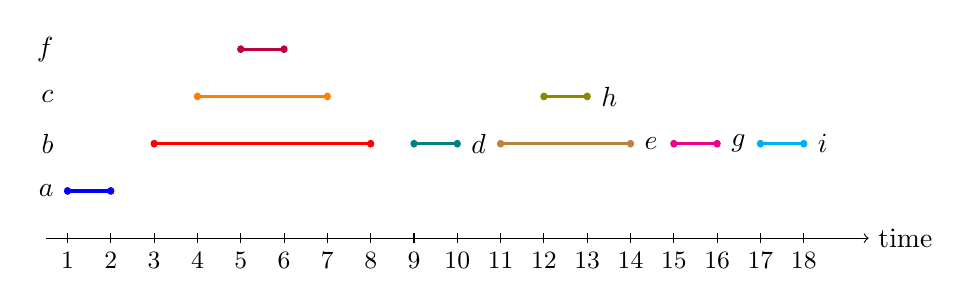
\begin{tikzpicture}[xscale=0.55, yscale=0.6]
  % Time axis
  \draw[->] (0.5, 0) -- (19.5, 0) node[right] {time};
  \foreach \t in {1,...,18} {
    \draw (\t, 0.1) -- (\t, -0.1) node[below] {\small \t};
  }

  % Node intervals [d, f] drawn as thick horizontal bars, stacked vertically
  % a: [1,2]
  \draw[very thick, blue] (1,1) -- (2,1);
  \node[left] at (0.9, 1) {$a$};
  \filldraw[blue] (1,1) circle (2pt);
  \filldraw[blue] (2,1) circle (2pt);

  % b: [3,8]
  \draw[very thick, red] (3,2) -- (8,2);
  \node[left] at (0.9, 2) {$b$};
  \filldraw[red] (3,2) circle (2pt);
  \filldraw[red] (8,2) circle (2pt);

  % c: [4,7]  (nested in b)
  \draw[very thick, orange] (4,3) -- (7,3);
  \node[left] at (0.9, 3) {$c$};
  \filldraw[orange] (4,3) circle (2pt);
  \filldraw[orange] (7,3) circle (2pt);

  % f: [5,6]  (nested in c)
  \draw[very thick, purple] (5,4) -- (6,4);
  \node[left] at (0.9, 4) {$f$};
  \filldraw[purple] (5,4) circle (2pt);
  \filldraw[purple] (6,4) circle (2pt);

  % d: [9,10]
  \draw[very thick, teal] (9,2) -- (10,2);
  \node[right] at (10.1, 2) {$d$};
  \filldraw[teal] (9,2) circle (2pt);
  \filldraw[teal] (10,2) circle (2pt);

  % e: [11,14]
  \draw[very thick, brown] (11,2) -- (14,2);
  \node[right] at (14.1, 2) {$e$};
  \filldraw[brown] (11,2) circle (2pt);
  \filldraw[brown] (14,2) circle (2pt);

  % h: [12,13] (nested in e)
  \draw[very thick, olive] (12,3) -- (13,3);
  \node[right] at (13.1, 3) {$h$};
  \filldraw[olive] (12,3) circle (2pt);
  \filldraw[olive] (13,3) circle (2pt);

  % g: [15,16]
  \draw[very thick, magenta] (15,2) -- (16,2);
  \node[right] at (16.1, 2) {$g$};
  \filldraw[magenta] (15,2) circle (2pt);
  \filldraw[magenta] (16,2) circle (2pt);

  % i: [17,18]
  \draw[very thick, cyan] (17,2) -- (18,2);
  \node[right] at (18.1, 2) {$i$};
  \filldraw[cyan] (17,2) circle (2pt);
  \filldraw[cyan] (18,2) circle (2pt);

\end{tikzpicture}
\end{center}

The nesting reflects the DFS forest structure: $f \subset c \subset b$ (one tree), $h \subset e$ (another tree), and $a$, $d$, $g$, $i$ are roots of their own singleton or small trees.

%

\end{parts}

%%%

\question[5] Given a digraph $G$, we can create its \textit{transpose}, called $G^T$, by reversing all of $G$'s edges. E.g. $(u, v) \in G.E$ if and only if $(v, u) \in G^{T}.E$.

Give an example of a non-empty digraph $G$ such that $G = G^T$, meaning that the transpose would have the exact same nodes and edges as the original graph.

\textbf{Solution:}

Let $G = (\{u, v\},\; \{(u,v),\,(v,u)\})$, i.e.\ two nodes with directed edges going in both directions:

\begin{center}
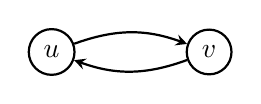
\begin{tikzpicture}[->, >=stealth, auto, node distance=2cm, thick]
  \node[circle, draw] (u) {$u$};
  \node[circle, draw] (v) [right of=u] {$v$};
  \path (u) edge[bend left=20] (v);
  \path (v) edge[bend left=20] (u);
\end{tikzpicture}
\end{center}

Transposing reverses $(u,v) \to (v,u)$ and $(v,u) \to (u,v)$, which gives back the same edge set. Therefore $G = G^T$.

More generally, any digraph consisting entirely of symmetric edge pairs (for every $(u,v)$, also $(v,u)$) and/or self-loops satisfies $G = G^T$.

%%%

\question Assume BFS outputted this predecessor table when run on some graph $G$:

\begin{tabular}{c | c}
Node & $p$ \\
\hline
p & NIL \\
q & s \\
r & u \\
s & v \\
t & q \\
u & p \\
v & p \\
\end{tabular}

\begin{parts}

%

\part[3] Give the shortest path from $p$ to $t$ and its length.

\textbf{Solution:}

Trace predecessors backwards from $t$:
\[
t \xrightarrow{p} q \xrightarrow{p} s \xrightarrow{p} v \xrightarrow{p} p
\]

Reversing gives the shortest path: $p \to v \to s \to q \to t$.

\textbf{Length:} 4 edges.

%

\part[2] Does this predecessor table contain all edges in $G$? Why or why not?

\textbf{Solution:}

No. The predecessor table only records the \textit{BFS tree edges} --- the edges BFS actually used to first discover each node. BFS may encounter many edges that lead to already-discovered (GRAY or BLACK) nodes; those edges are never stored in $p$. For example, $G$ could contain an edge $(p, q)$ directly, but since $q$ was first discovered via $s$, we have $q.p = s$ and the edge $(p, q)$ does not appear in the table. In general there can be many more edges in $G$ than the $|V|-1$ tree edges shown here.

%

\end{parts}

%%%

\question The CS department is planning a curriculum redesign. Each CS course $x$ has 0 or more CS courses as prerequisites, which must all be taken before $x$.

You've been asked to design an algorithm that will check if, given each CS course and its prerequisites, there's any sequence of courses that would be impossible to take in any order.

\begin{parts}

%

\part[5] Describe how you'd model this problem as a graph by answering all of the following questions:

\begin{itemize}
\item What are the nodes?
\item What does an edge between two nodes represent about those nodes?
\item Is the graph directed or undirected?
\item Is the graph weighted or unweighted? If weighted, what are the weights?
\end{itemize}

\textbf{Solution:}

\begin{itemize}
  \item \textbf{Nodes:} Each CS course is a node.
  \item \textbf{Edges:} A directed edge $(u, v)$ means course $u$ is a prerequisite of course $v$ (i.e.\ $u$ must be taken before $v$).
  \item \textbf{Directed.} The prerequisite relationship is not symmetric: if $u$ must be taken before $v$, it does not mean $v$ must be taken before $u$.
  \item \textbf{Unweighted.} We only care about the existence of prerequisite relationships, not any numeric weight between them.
\end{itemize}

%

\part[15] Design an algorithm that takes the graph you previously described as input and outputs false if the graph has an impossible preqrequisite sequence and true otherwise. Briefly explain why your algorithm solves the problem.

If your algorithm reuses other algorithms given in the class with some tweaks, reproduce their pseudocode in full with any changes you might've made.

\textbf{Solution:}

\textbf{High-level idea:} A sequence of courses is impossible if and only if the prerequisite graph contains a \textit{cycle} (e.g.\ course A requires B, B requires C, C requires A — none can ever be taken first). We detect cycles using DFS: a back edge --- an edge to a currently GRAY (in-progress) ancestor --- indicates a cycle. If no back edge is found, the graph is a DAG and all courses can be ordered via topological sort.

\begin{verbatim}
function HasValidOrdering(graph):
    global time = 0

    for u in graph.vertices:
        u.color = WHITE
        u.p = NIL

    for u in graph.vertices:
        if u.color == WHITE:
            if CycleFound(graph, u):
                return false   // cycle exists => impossible sequence

    return true   // no cycle => valid ordering exists


function CycleFound(graph, u):
    time++
    u.d = time
    u.color = GRAY

    for v in graph.adjacencyList[u]:
        if v.color == GRAY:
            return true        // back edge found => cycle
        if v.color == WHITE:
            v.p = u
            if CycleFound(graph, v):
                return true

    u.color = BLACK
    time++
    u.f = time
    return false
\end{verbatim}

\textbf{Why it works:} By the DFS white-path theorem, a back edge $(u, v)$ (where $v$ is GRAY, meaning it is an ancestor of $u$ on the current DFS path) exists if and only if the graph has a cycle. If a cycle exists, some set of courses has a circular prerequisite dependency and no valid enrollment order exists, so we return \texttt{false}. If DFS completes without finding any back edge, the graph is a DAG and a topological ordering (valid course sequence) exists, so we return \texttt{true}.

\part[5] Give tight bounds on the best and worst case runtimes of your algorithm and briefly justify your bounds.

\textbf{Solution:}

Let $V$ be the number of courses and $E$ the number of prerequisite edges.

\textbf{Best case: $\Theta(V)$.} The initialization loop always runs in $\Theta(V)$. In the best case, a cycle is detected immediately upon encountering the first back edge (e.g.\ a self-loop on the first node visited), so only $O(1)$ additional work is done after initialization. The total is $\Theta(V)$.

\textbf{Worst case: $\Theta(V + E)$.} In the worst case the graph is a DAG (no cycle), so DFS runs to completion --- visiting every vertex and examining every edge exactly once. This matches standard DFS complexity: $\Theta(V + E)$.

\end{parts}

%%%

\question Consider a 2D grid where each square represents either water or land. For example, in the below 8x7 grid, each tan square is a land square and each blue square is a water square (the numbers on the outside of the grid label the indices of each square):

\textit{Image removed from student template}

If two land squares are vertically or horizontally (but not diagonally) adjacent, they are considered to be part of the same island. There are four islands in this grid (given different colors below):

\textit{Image removed from student template}

The purple island on $(5, 2)$ and the orange island on $(6, 1)$ are considered separate because they're only diagonally adjacent, not vertically or horizontally adjacent.

\begin{parts}

%

\part[15] Design an algorithm that will take an $n \times m$ array of booleans, where true means the square is an island and false means it's water, and a $(row, column)$ pair of indices. It should return a count of the number of squares in the island the $(row, column)$ pair is a part of, if any.

For example, when given the above grid and $(3, 1)$ as input, your algorithm should return 17. If given $(6, 1)$ as input, your algorithm should return 1. If given $(3, 4)$ as input, your algorithm should return 0.

If your algorithm reuses other algorithms given in the class with some tweaks, you \textbf{don't} have to reproduce their pseudocode in full -- just describe in detail any changes you'd make.

Hint: How could you convert the inputted 2D array of booleans into a graph, whether an adjacency matrix or adjacency list? What would be your vertices and their labels? How would you represent edges? Note that each $(row, column)$ cell can be given a unique label of $row * n + column$.

\textbf{Solution:}

\textbf{Graph model:} Each land cell $(r, c)$ is a vertex with unique label $r \times m + c$ (using $m$ as the number of columns to guarantee uniqueness). There is an undirected edge between two cells if and only if they are horizontally or vertically adjacent and \textit{both} are land. We represent this implicitly via the grid itself rather than building an explicit adjacency structure.

\textbf{High-level idea:} If the starting cell is water, immediately return 0. Otherwise, run a DFS from the starting cell, counting every land cell visited. We use a \texttt{visited} array to avoid revisiting cells (equivalent to the WHITE/GRAY/BLACK coloring in standard DFS).

\begin{verbatim}
function islandSize(grid, startRow, startCol):
    n = number of rows in grid
    m = number of columns in grid

    if grid[startRow][startCol] == false:
        return 0

    visited = 2D boolean array of size n x m, initialized to false
    return DFSCount(grid, visited, startRow, startCol, n, m)


function DFSCount(grid, visited, row, col, n, m):
    // Out of bounds check
    if row < 0 or row >= n or col < 0 or col >= m:
        return 0
    // Water or already visited
    if grid[row][col] == false or visited[row][col] == true:
        return 0

    visited[row][col] = true
    count = 1

    // Recurse into four cardinal neighbors
    count += DFSCount(grid, visited, row - 1, col, n, m)  // up
    count += DFSCount(grid, visited, row + 1, col, n, m)  // down
    count += DFSCount(grid, visited, row, col - 1, n, m)  // left
    count += DFSCount(grid, visited, row, col + 1, n, m)  // right

    return count
\end{verbatim}

This is standard DFS with two modifications: (1) the ``graph'' is implicit in the grid, so instead of iterating over an adjacency list we check the four cardinal neighbors directly; (2) we count visited land nodes rather than recording timestamps.

%

\part[10] Give tight bounds on the best and worst case running times of your algorithm in terms of $n$ and $m$ and briefly justify your bounds.

\textbf{Solution:}

\textbf{Best case: $\Theta(1)$.} If the starting cell is water (\texttt{grid[startRow][startCol] == false}), the algorithm returns 0 immediately after a single array lookup --- no DFS is started and no \texttt{visited} array needs to be allocated. This is $\Theta(1)$.

\textbf{Worst case: $\Theta(n \cdot m)$.} In the worst case, the entire grid is one large island and the starting cell is a land cell. DFS visits every cell exactly once (the \texttt{visited} check ensures no cell is processed more than once), and for each cell it examines at most 4 neighbors. Initializing the \texttt{visited} array costs $\Theta(n \cdot m)$. The total work is therefore $\Theta(n \cdot m)$.

\end{parts}

%%%

\end{questions}

\end{document}
